We have installed a Jupyter server as a component of our MathHub system.
It provides a normal Jupyter server except for additionally supporting our MMT kernel.
It is available at the URL \url{jupyter.mathhub.info}.\ednote{@Kai: check this}

MathHub.info is backed by Git repositories, in which we store Jupyter notebooks as regular files.
The frontend can provide special interaction functionality for individual document types.
We have now added Jupyter notebooks as a new document type.%
\footnote{The MathHub front-end is currently undergoing a major re-write.
The old MathHub interface was based on Drupal, which led to major system vulnerabilities and therefore maintenance hassles, because Drupal was targeted by hackers.
We are currently working on a docker-based orchestration of services with a React.JS based front-end in the general spirit of the OpenDreamKit VRE toolkit; see \url{https://github.com/MathHubInfo/}. The new system can be accessed at \url{http://new.mathhub.info}.};
see Figure~\ref{fig:mathhub-NB} for an example.
When displaying a know document type in the MathHub front-end, multiple tabs are shown.
For notebooks, these are the following:
\begin{compactenum}
\item \textsf{view} gives a preview of the notebook, essentially the computation cells without output, prerendered for static serving without involving Jupyter at all.%
\ednote{MK: we should implement this; I am not sure what the best way is for this. I guess a build target based on \texttt{https://github.com/jendas1/jupyter-notebook-quick-look}.}
\item \textsf{run/edit} opens the respective notebook on \url{jupyter.mathhub.info} for execution and editing.
Any changes to the notebook can be committed back to the Git repository. 
\item \textsf{metadata} (this is the tab open in Figure~\ref{fig:mathhub-NB}), shows the metadata provided by the Jupyter kernel and the repository. 
\item \textsf{source} provides access to the document source; here simply a link to the notebook file in the Git repository.
\item \textsf{statistics} shows statistical information about the notebook, its corresponding MMT document, and its connections with other MMT documents in the background knowledge base.
\item \textsf{graph} links to graph-based visualizations of the document including the theory graph, declaration graph, and dependency graph, using our TGView system, a canvas-based in-browser visualizer for knowledge graph information~\cite{RupKohMue:fitgv17}.
\end{compactenum}
This integration combines the interactive features of the Jupyter server with the knowledge management facilities on MathHub.info. In the future, we plan to integrate the notebook diff/patch \textsf{nbdime} developed in OpenDreamKit to extend the knowledge management facilities. 

\begin{figure}[ht]\centering
  \fbox{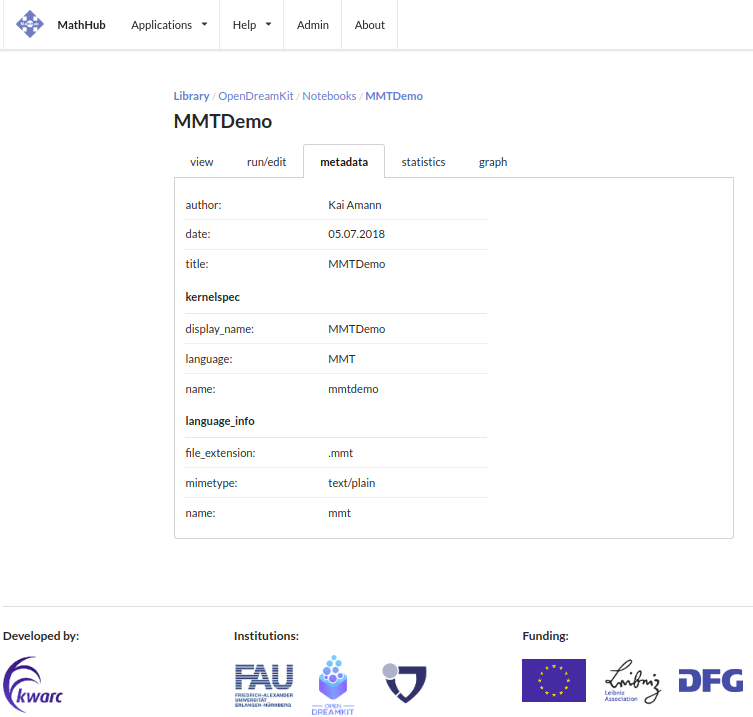
\includegraphics[width=13cm]{NB-Mathhub}}
  \caption{A Jupyter Notebook in MathHub.info (Metadata)}\label{fig:mathhub-NB}
\end{figure}

%A Jupyter Notebook additionally has a special button appears that allows users to open the notebook in the associated Jupyter server. Currently these notebooks do not use the MMT process running on MathHub.info, due to the architecture of the MMT Kernel. Therefore they currently do not have access to the MathHub universe. \ednote{KA: if the Kernel server would run on the same VM as the MathHub MMT we could give the kernel access to it}
%\ednote{@Kai, @Tom: check this, do the implementation}

\ednote{@KA: write the example from Fig.~\ref{fig:test_theory} as a Jupyter notebook, store the file somewhere on gl.mathhub.info and give a link to the Fig.~\ref{fig:mathhub-NB} view of that notebook}


%%% Local Variables:
%%% mode: latex
%%% mode: visual-line
%%% fill-column: 5000
%%% TeX-master: "report"
%%% End:

%  LocalWords:  Jupyter ednote
